% Source slide 1
\section[4.1 Vector Spaces]{4.1 Vector Spaces and Subspaces}
\chaptercard{4}{Vector Spaces}{4.1}{VECTOR SPACES AND SUBSPACES}

% Source slide 2
\begin{frame}{Overview of Linear Algebra}
\centering
\Large
\begin{align*}
\text{平面（2维）解析几何} &\Longleftrightarrow \R^2\text{的线性代数},\\
\text{空间（3维）解析几何} &\Longleftrightarrow \R^3\text{的线性代数},\\
\text{$n$维数组空间解析几何} &\Longleftrightarrow \R^n\text{的线性代数}.
\end{align*}
\vspace{0.4cm}
\begin{tikzpicture}[>=Stealth,thick]
  \node[draw,fill=yellow,minimum width=4.8cm,minimum height=1.0cm] (v) {一般的向量空间};
  \node[right=5.5cm of v] (m) {矩阵的运算};
  \draw[<->,line width=2pt,draw=pink!60!black] ($(v.north)+(0,0.2)$) -- node[right,black]{\Large\itshape Basis} ++(0,1.8);
  \draw[<->,line width=2pt,draw=pink!60!black] ($(m.north)+(0,0.2)$) -- ++(0,1.8);
\end{tikzpicture}
\end{frame}

% Source slide 3
\begin{frame}[shrink=11]{VECTOR SPACES AND SUBSPACES}
\begin{itemize}
\item \textbf{Definition:} A \textcolor{blue!60}{\textbf{vector space}} is a nonempty set $V$ of objects, called \emph{vectors}, on which are defined two operations, called \emph{addition and multiplication by scalars} (real numbers), subject to the ten axioms (or rules) listed below. The axioms must hold for all vectors $\vect u$, $\vect v$, and $\vect w$ in $V$ and for all scalars $c$ and $d$.
\end{itemize}
\begin{enumerate}
\item The sum of $\vect u$ and $\vect v$, denoted by $\vect u+\vect v$, is in $V$.
\item $\vect u+\vect v=\vect v+\vect u$.
\item $(\vect u+\vect v)+\vect w=\vect u+(\vect v+\vect w)$.
\item There is a zero vector $0$ in $V$ such that
\[
\vect u+0=\vect u.
\]
\end{enumerate}
\end{frame}

% Source slide 4
\begin{frame}[shrink=9]{VECTOR SPACES AND SUBSPACES}
\begin{enumerate}
\setcounter{enumi}{4}
\item For each $\vect u$ in $V$, there is a vector $-\vect u$ in $V$ such that $\vect u+(-\vect u)=0$.
\item The scalar multiple of $\vect u$ by $c$, denoted by $c\vect u$, is in $V$.
\item $c(\vect u+\vect v)=c\vect u+c\vect v$.
\item $(c+d)\vect u=c\vect u+d\vect u$.
\item $c(d\vect u)=(cd)\vect u$.
\item $1\vect u=\vect u$.
\end{enumerate}
\begin{itemize}
\item Using these axioms, we can show that \textcolor{red}{the zero vector in Axiom 4 is unique}, and the vector $-\vect u$, called the \textbf{negative} of $\vect u$, in Axiom 5 is unique for each $\vect u$ in $V$.
\end{itemize}
\end{frame}

% Source slide 5
\begin{frame}[shrink=8]{VECTOR SPACES AND SUBSPACES}
\begin{itemize}
\item For each $\vect u$ in $V$ and scalar $c$,
\end{itemize}
\begin{align}
0\vect u&=0 \tag{1}\\
c0&=0 \tag{2}\\
-\vect u&=(-1)\vect u. \tag{3}
\end{align}
\vspace{0.6cm}
{\Large\color{sourcecyan}Examples --- Vector Spaces of Real Number Vectors}
\medskip

\textcolor{red!70!black}{\textbf{EXAMPLE 1}}\quad
The spaces $\R^n$, where $n\geq1$, are the premier examples of vector spaces. The geometric intuition developed for $\R^3$ will help you understand and visualize many concepts throughout the chapter.
\end{frame}

% Source slide 6
\begin{frame}[shrink=12]{Examples --- Vector Spaces of Arrows}
\begin{itemize}
\item \textbf{Example 2:} Let $V$ be the set of all arrows (directed line segments) in three-dimensional space, with two arrows regarded as equal if they have the same length and point in the same direction. Define addition by the parallelogram rule, and for each $\vect v$ in $V$, define $c\vect v$ to be the arrow whose length is $c$ times the length of $\vect v$, pointing in the same direction as $\vect v$ if $c\geq0$ and otherwise pointing in the opposite direction.
\item See the following figure below. Show that $V$ is a vector space.
\end{itemize}
\centering
\begin{tikzpicture}[>=Stealth,scale=0.9]
  \draw[->,very thick,cyan] (0,0)--(0.55,1.25) node[midway,left,black] {$\vect v$};
  \draw[->,very thick,cyan] (2,0)--(3.25,2.85) node[midway,left,black] {$3\vect v$};
  \draw[->,very thick,cyan] (5.2,1.5)--(4.7,0.35) node[midway,left,black] {$-\vect v$};
\end{tikzpicture}
\end{frame}

% Source slide 7
\begin{frame}[shrink=13]
\begin{itemize}
\item \textbf{Solution:} The definition of $V$ is geometric, using concepts of length and direction.
\item No $x\ y\ z$-coordinate system is involved.
\item An arrow of zero length is a single point and represents the zero vector.
\item The negative of $\vect v$ is $-\vect v$.
\item So Axioms 1, 4, 5, 6, and 10 are evident. See the figures on the next slide.
\end{itemize}
\begin{columns}[T]
\column{.48\textwidth}
\centering
\begin{tikzpicture}[>=Stealth,scale=0.62]
  \coordinate (A) at (0,0); \coordinate (B) at (1.2,2.6); \coordinate (C) at (6.0,3.2); \coordinate (D) at (4.8,0.8);
  \draw[->,thick] (A)--(B) node[midway,left] {$\vect u$};
  \draw[->,thick] (D)--(C) node[midway,right] {$\vect u$};
  \draw[->,thick] (B)--(D) node[midway,below] {$\vect v$};
  \draw[->,very thick,cyan] (A)--(D) node[midway,below] {$\vect u+\vect v$};
  \draw[->,very thick,cyan] (B)--(C) node[midway,above] {$\vect v+\vect u$};
\end{tikzpicture}

$\vect u+\vect v=\vect v+\vect u$.
\column{.48\textwidth}
\centering
\begin{tikzpicture}[>=Stealth,scale=0.58]
  \coordinate (A) at (0,0); \coordinate (B) at (1.0,2.3); \coordinate (C) at (5.5,3.3); \coordinate (D) at (6.8,0.9);
  \draw[->,thick] (A)--(B) node[midway,left] {$\vect u$};
  \draw[->,thick] (B)--(C) node[midway,above] {$\vect v$};
  \draw[->,thick] (C)--(D) node[midway,right] {$\vect w$};
  \draw[->,very thick,cyan] (A)--(C) node[midway,below] {$\vect u+\vect v$};
  \draw[->,very thick,cyan] (B)--(D) node[midway,below] {$\vect v+\vect w$};
  \draw[->,very thick,cyan] (A)--(D) node[midway,below] {$\vect u+\vect v+\vect w$};
\end{tikzpicture}

$(\vect u+\vect v)+\vect w=\vect u+(\vect v+\vect w)$.
\end{columns}
\end{frame}

% Source slide 8
\begin{frame}[shrink=24]{Examples --- Vector Spaces of Functions}
\textcolor{red!70!black}{\textbf{EXAMPLE 5}}\quad
Let $V$ be the set of all real-valued functions defined on a set $\mathbb D$. (Typically, $\mathbb D$ is the set of real numbers or some interval on the real line.) Functions are added in the usual way: $\vect f+\vect g$ is the function whose value at $t$ in the domain $\mathbb D$ is $f(t)+g(t)$. Likewise, for a scalar $c$ and an $\vect f$ in $V$, the scalar multiple $c\vect f$ is the function whose value at $t$ is $cf(t)$. For instance, if $\mathbb D=\R$, $f(t)=1+\sin 2t$, and $g(t)=2+.5t$, then
\[
(\vect f+\vect g)(t)=3+\sin 2t+.5t
\qquad\text{and}\qquad
(2\vect g)(t)=4+t.
\]
Two functions in $V$ are equal if and only if their values are equal for every $t$ in $\mathbb D$. Hence the zero vector in $V$ is the function that is identically zero, $f(t)=0$ for all $t$, and the negative of $\vect f$ is $(-1)\vect f$. Axioms 1 and 6 are obviously true, and the other axioms follow from properties of the real numbers, so $V$ is a vector space.

\begin{center}
\begin{tikzpicture}[>=Stealth,scale=0.65]
  \coordinate (O) at (0,0); \coordinate (F) at (-0.5,1.7); \coordinate (G) at (1.1,0.9); \coordinate (S) at (0.6,2.6);
  \fill[cyan!25] (O)--(F)--(S)--(G)--cycle;
  \fill[cyan] (O) circle (2pt) node[below] {$0$};
  \fill[cyan] (F) circle (2pt) node[left] {$\vect f$};
  \fill[cyan] (G) circle (2pt) node[right] {$\vect g$};
  \fill[cyan] (S) circle (2pt) node[right] {$\vect f+\vect g$};
\end{tikzpicture}

\textbf{FIGURE 5}\quad The sum of two vectors (functions).
\end{center}
\end{frame}

% Source slide 9
\begin{frame}[shrink=9]{SUBSPACES}
\begin{itemize}
\item \textbf{Definition:} A \textbf{subspace} of a vector space $V$ is a subset $H$ of $V$ that has three properties:
\end{itemize}
\begin{enumerate}
\item[(a.)] The zero vector of $V$ is in $H$.
\item[(b.)] $H$ is closed under vector addition. That is, for each $\vect u$ and $\vect v$ in $H$, the sum $\vect u+\vect v$ is in $H$.
\item[(c.)] $H$ is closed under multiplication by scalars. That is, for each $\vect u$ in $H$ and each scalar $c$, the vector $c\vect u$ is in $H$.
\end{enumerate}
\end{frame}

% Source slide 10
\begin{frame}{SUBSPACES}
\begin{itemize}
\item Properties (a), (b), and (c) guarantee that a subspace $H$ of $V$ is itself a \emph{vector space}, under the vector space operations already defined in $V$.
\item Every subspace is a vector space.
\item Conversely, every \emph{vector space} is a subspace (of itself and possibly of other larger spaces).
\end{itemize}
\end{frame}

% Source slide 11
\begin{frame}[shrink=10]
\textcolor{red!70!black}{\textbf{EXAMPLE 6}}\quad
The set consisting of only the zero vector in a vector space $V$ is a subspace of $V$, called the \textbf{zero subspace} and written as $\{0\}$.
\vspace{0.5cm}
\begin{columns}[T]
\column{.48\textwidth}
\centering
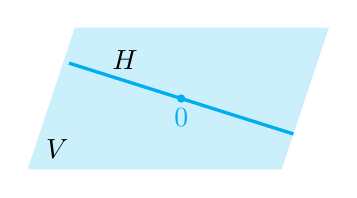
\begin{tikzpicture}[scale=0.75]
  \fill[cyan!20] (0,0)--(4.3,0)--(5.1,2.4)--(0.8,2.4)--cycle;
  \draw[cyan,very thick] (0.7,1.8)--(4.5,0.6) node[pos=.25,above,black] {$H$};
  \fill[cyan] (2.6,1.2) circle (2pt) node[below] {$0$};
  \node at (.5,.35) {$V$};
\end{tikzpicture}

\textbf{FIGURE 6}\par A subspace of $V$.
\column{.48\textwidth}
\centering
\begin{tikzpicture}[>=Stealth,scale=0.58]
  \fill[green!45] (-2,-1)--(2.8,-.4)--(2,1.5)--(-2.8,.8)--cycle;
  \draw[->] (-3,0)--(3,0) node[right] {$x_2$};
  \draw[->] (-2,-1.5)--(2,1.8) node[above] {$x_1$};
  \draw[->] (0,-1.6)--(0,2) node[above] {$x_3$};
  \node at (1,-.3) {$H$};
\end{tikzpicture}

\textbf{FIGURE 7}\par The $x_1x_2$-plane as a subspace of $\R^3$.
\end{columns}
\end{frame}

% Source slide 12
\begin{frame}[shrink=11]
\textcolor{red!70!black}{\textbf{EXAMPLE 9}}\quad
A plane in $\R^3$ \emph{not} through the origin is not a subspace of $\R^3$, because the plane does not contain the zero vector of $\R^3$. Similarly, a line in $\R^2$ \emph{not} through the origin, such as in Figure 8, is not a subspace of $\R^2$.
\vspace{0.7cm}
\begin{center}
\begin{tikzpicture}[>=Stealth,scale=0.8]
  \draw[->] (-2.2,0)--(2.4,0) node[right] {$x_1$};
  \draw[->] (0,-1.2)--(0,2.2) node[above] {$x_2$};
  \draw[cyan,very thick] (-1.5,1.4)--(1.8,-.7) node[midway,above] {$H$};
\end{tikzpicture}

\textbf{FIGURE 8}\par A line that is not a vector space.
\end{center}
\end{frame}

% Source slide 13
\begin{frame}{A SUBSPACE SPANNED BY A SET}
\begin{itemize}
\item ------ \textcolor{cyan}{\emph{the most common ways of describing a subspace}}
\item As the term \textcolor{sourceblue}{\textbf{linear combination}} refers to any sum of scalar multiples of vectors, and \textcolor{sourceblue}{\textbf{$\Span\{\vect v_1,\ldots,\vect v_p\}$}} denotes the set of all vectors that can be written as linear combinations of $\vect v_1,\ldots,\vect v_p$.
\end{itemize}
\end{frame}

% Source slide 14
\begin{frame}[shrink=14]{A SUBSPACE SPANNED BY A SET}
\begin{itemize}
\item \textbf{Example 10:} Given $\vect v_1$ and $\vect v_2$ in a vector space $V$, let $H=\Span\{\vect v_1,\vect v_2\}$. Show that $H$ is a subspace of $V$.
\item \textbf{Solution:} The zero vector is in $H$, since $0=0\vect v_1+0\vect v_2$.
\item To show that $H$ is closed under vector addition, take two arbitrary vectors in $H$, say,
\[
\vect u=s_1\vect v_1+s_2\vect v_2
\qquad\text{and}\qquad
\vect w=t_1\vect v_1+t_2\vect v_2.
\]
\item By Axioms 2, 3, and 8 for the vector space $V$,
\begin{align*}
\vect u+\vect w&=(s_1\vect v_1+s_2\vect v_2)+(t_1\vect v_1+t_2\vect v_2)\\
&=(s_1+t_1)\vect v_1+(s_2+t_2)\vect v_2.
\end{align*}
\end{itemize}
\end{frame}

% Source slide 15
\begin{frame}[shrink=13]{A SUBSPACE SPANNED BY A SET}
\begin{itemize}
\item So $\vect u+\vect w$ is in $H$.
\item Furthermore, if $c$ is any scalar, then by Axioms 7 and 9,
\[
c\vect u=c(s_1\vect v_1+s_2\vect v_2)=(cs_1)\vect v_1+(cs_2)\vect v_2,
\]
which shows that $c\vect u$ is in $H$ and $H$ is closed under scalar multiplication.
\item Thus $H$ is a subspace of $V$.
\end{itemize}
\begin{flushright}
\begin{tikzpicture}[>=Stealth,scale=0.52]
  \fill[cyan!20] (-3,-.7)--(2.7,-.4)--(3.2,.9)--(-2.5,.7)--cycle;
  \draw[->] (-3,0)--(3.2,0) node[right] {$x_2$};
  \draw[->] (-2,-1.4)--(2,1.4) node[above] {$x_1$};
  \draw[->] (0,-1)--(0,1.8) node[above] {$x_3$};
  \fill[cyan] (-.9,.1) circle (2pt) node[above] {$\vect v_1$};
  \fill[cyan] (1,.25) circle (2pt) node[above] {$\vect v_2$};
  \node at (0,.4) {$0$};
\end{tikzpicture}

\textbf{FIGURE 9}\quad An example of a subspace.
\end{flushright}
\end{frame}

% Source slide 16
\begin{frame}[shrink=9]{A SUBSPACE SPANNED BY A SET}
\begin{itemize}
\item \sourcehead{Theorem 1:} If $\vect v_1,\ldots,\vect v_p$ are in a vector space $V$, then $\Span\{\vect v_1,\ldots,\vect v_p\}$ is a subspace of $V$.
\item We call $\Span\{\vect v_1,\ldots,\vect v_p\}$ \textbf{the subspace spanned} (or \textbf{generated}) by $\{\vect v_1,\ldots,\vect v_p\}$.
\item Give any subspace $H$ of $V$, a \textbf{spanning} (or \textbf{generating}) set for $H$ is a set $\{\vect v_1,\ldots,\vect v_p\}$ in $H$ such that
\[
H=\Span\{\vect v_1,\ldots,\vect v_p\}.
\]
\end{itemize}
\end{frame}

% Source slide 17
\begin{frame}[shrink=18]
\textcolor{red!70!black}{\textbf{EXAMPLE 11}}\quad
Let $H$ be the set of all vectors of the form $(a-3b,b-a,a,b)$, where $a$ and $b$ are arbitrary scalars. That is, let
\[
H=\{(a-3b,b-a,a,b):a\text{ and }b\text{ in }\R\}.
\]
Show that $H$ is a subspace of $\R^4$.

\textcolor{red!70!black}{\textbf{SOLUTION}}\quad Write the vectors in $H$ as column vectors. Then an arbitrary vector in $H$ has the form
\[
\begin{bmatrix}a-3b\\b-a\\a\\b\end{bmatrix}
=a\underbrace{\begin{bmatrix}1\\-1\\1\\0\end{bmatrix}}_{\vect v_1}
+b\underbrace{\begin{bmatrix}-3\\1\\0\\1\end{bmatrix}}_{\vect v_2}.
\]
This calculation shows that $H=\Span\{\vect v_1,\vect v_2\}$, where $\vect v_1$ and $\vect v_2$ are the vectors indicated above. Thus $H$ is a subspace of $\R^4$ by Theorem 1.

\begin{center}
Calculations with the infinitely many vectors in $H$\\[-.2ex]
$\Updownarrow$\\[-.2ex]
Operations with the finite number of vectors in the spanning set.
\end{center}
\end{frame}
